% -*- root: ../thesis.tex -*-
%!TEX root = ../thesis.tex
% ******************************* Thesis Appendix A ****************************
\chapter{Additional works} 

The following works do not fit the storyline of the thesis and are presented here.
They include a solo project around the choice of inducing points and a joint work with a master student on evidence estimation using \ac{SVGD}.
They were not extended further due to a lack of time and/or inconclusive results.
Both were reviewed and accepted into workshops.


\section{Adaptive Inducing Points Selection for Gaussian Processes}

\textbf{\underlin{Authors:}}\\
Th\'eo Galy-Fajou$^1$, Manfred Opper$^1$
\small{$^1$TU Berlin}

\textbf{\underline{Details:}}\\
Type: Workshop article
Submitted: June 2020\\
Accepted: July 2020\\
URL: \url{https://drive.google.com/file/d/1IPTUBfY_b2WElTWBIVU4lrbHcXnbTWdB/view}\\
Conference: Workshop Continual Learning (ICML 2020)\\


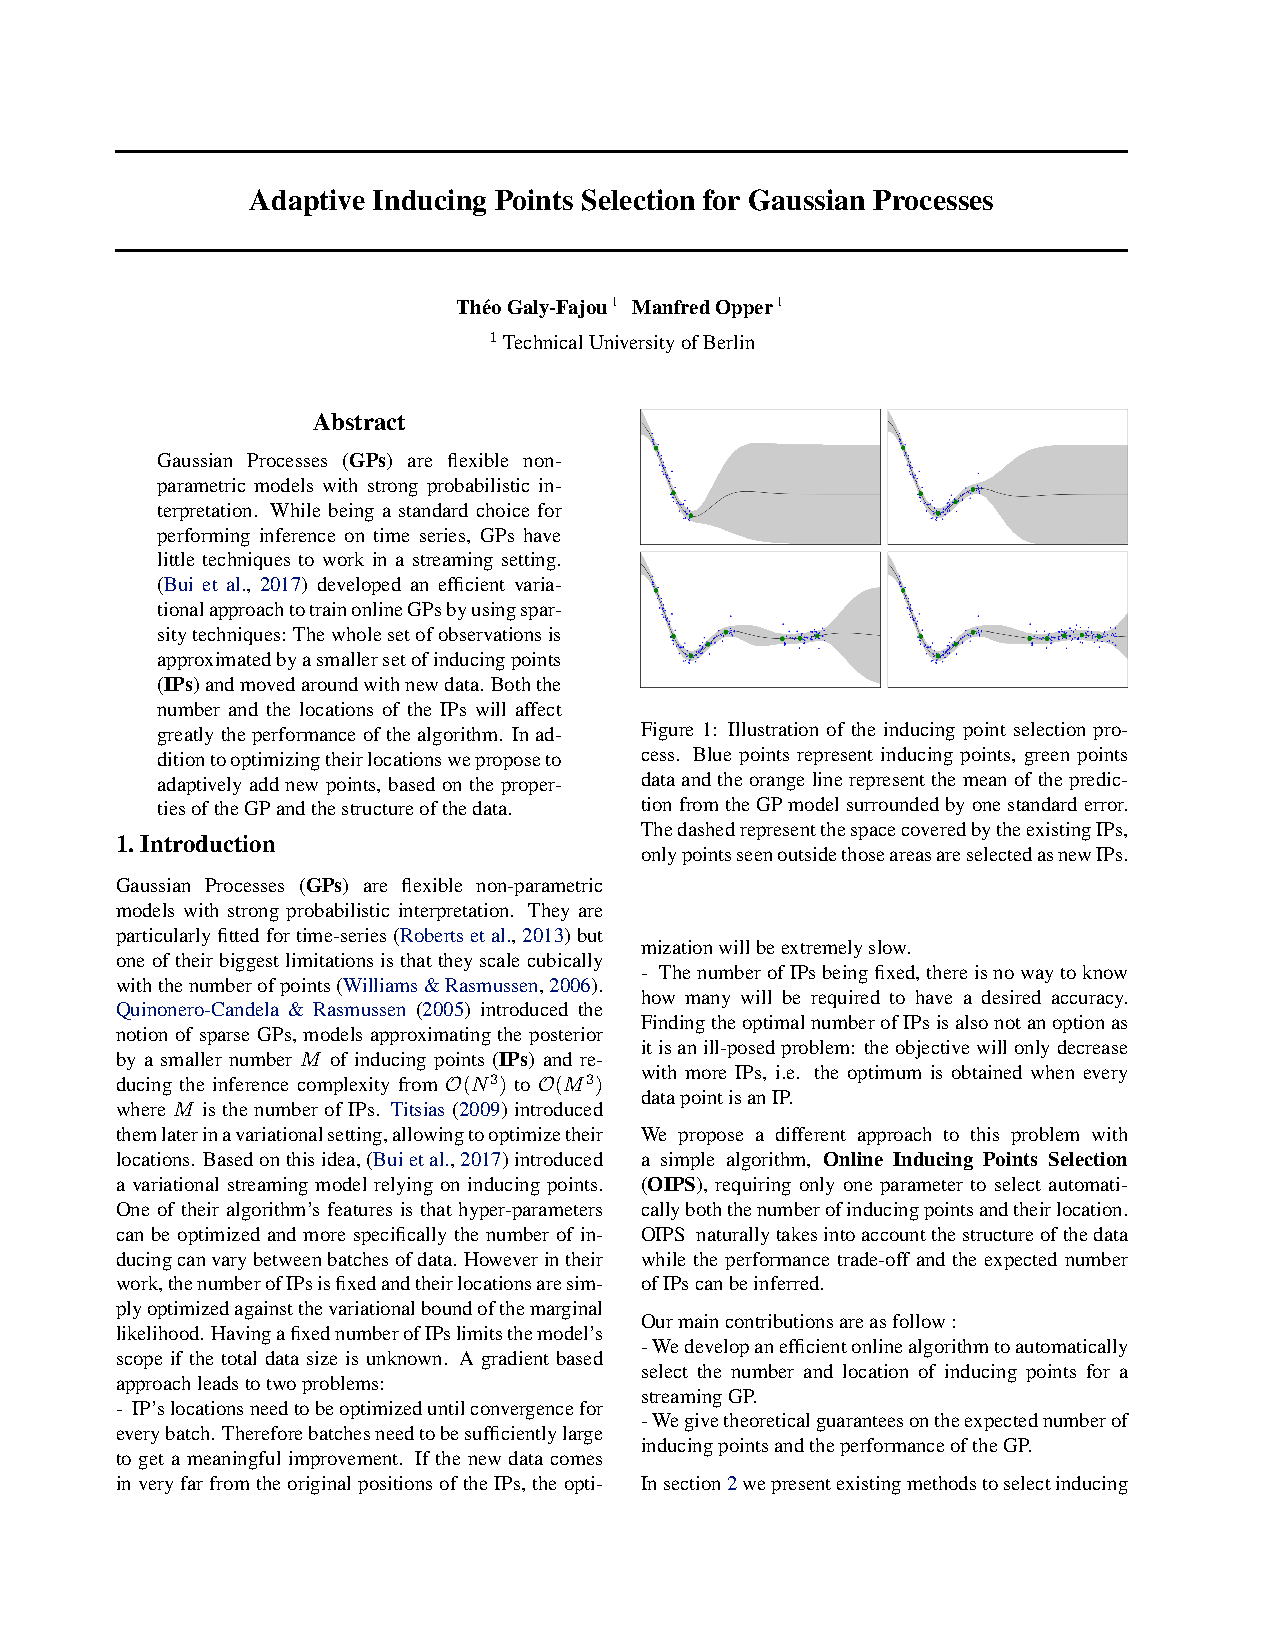
\includepdf[pages=-,pagecommand={},scale=0.95]{28_CameraReadySubmission_cl_workshop_onlinegp.pdf}

\section{Evidence Estimation by Kullback-Leibler Integration for Flow-Based Methods}

\textbf{\underlin{Authors:}}\\
Nikolai ZakiR$^1$, Th\'eo Galy-Fajou$^1$, Manfred Opper$^1$
\small{$^1$TU Berlin}

\textbf{\underline{Details:}}\\
Type: Workshop article
Submitted: October 2020\\
Accepted: December 2020\\
URL : \url{https://openreview.net/forum?id=LclKtSfmf9I}\\
Conference: 3rd Symposium on Advances in Approximate Bayesian Inference, 2020\\


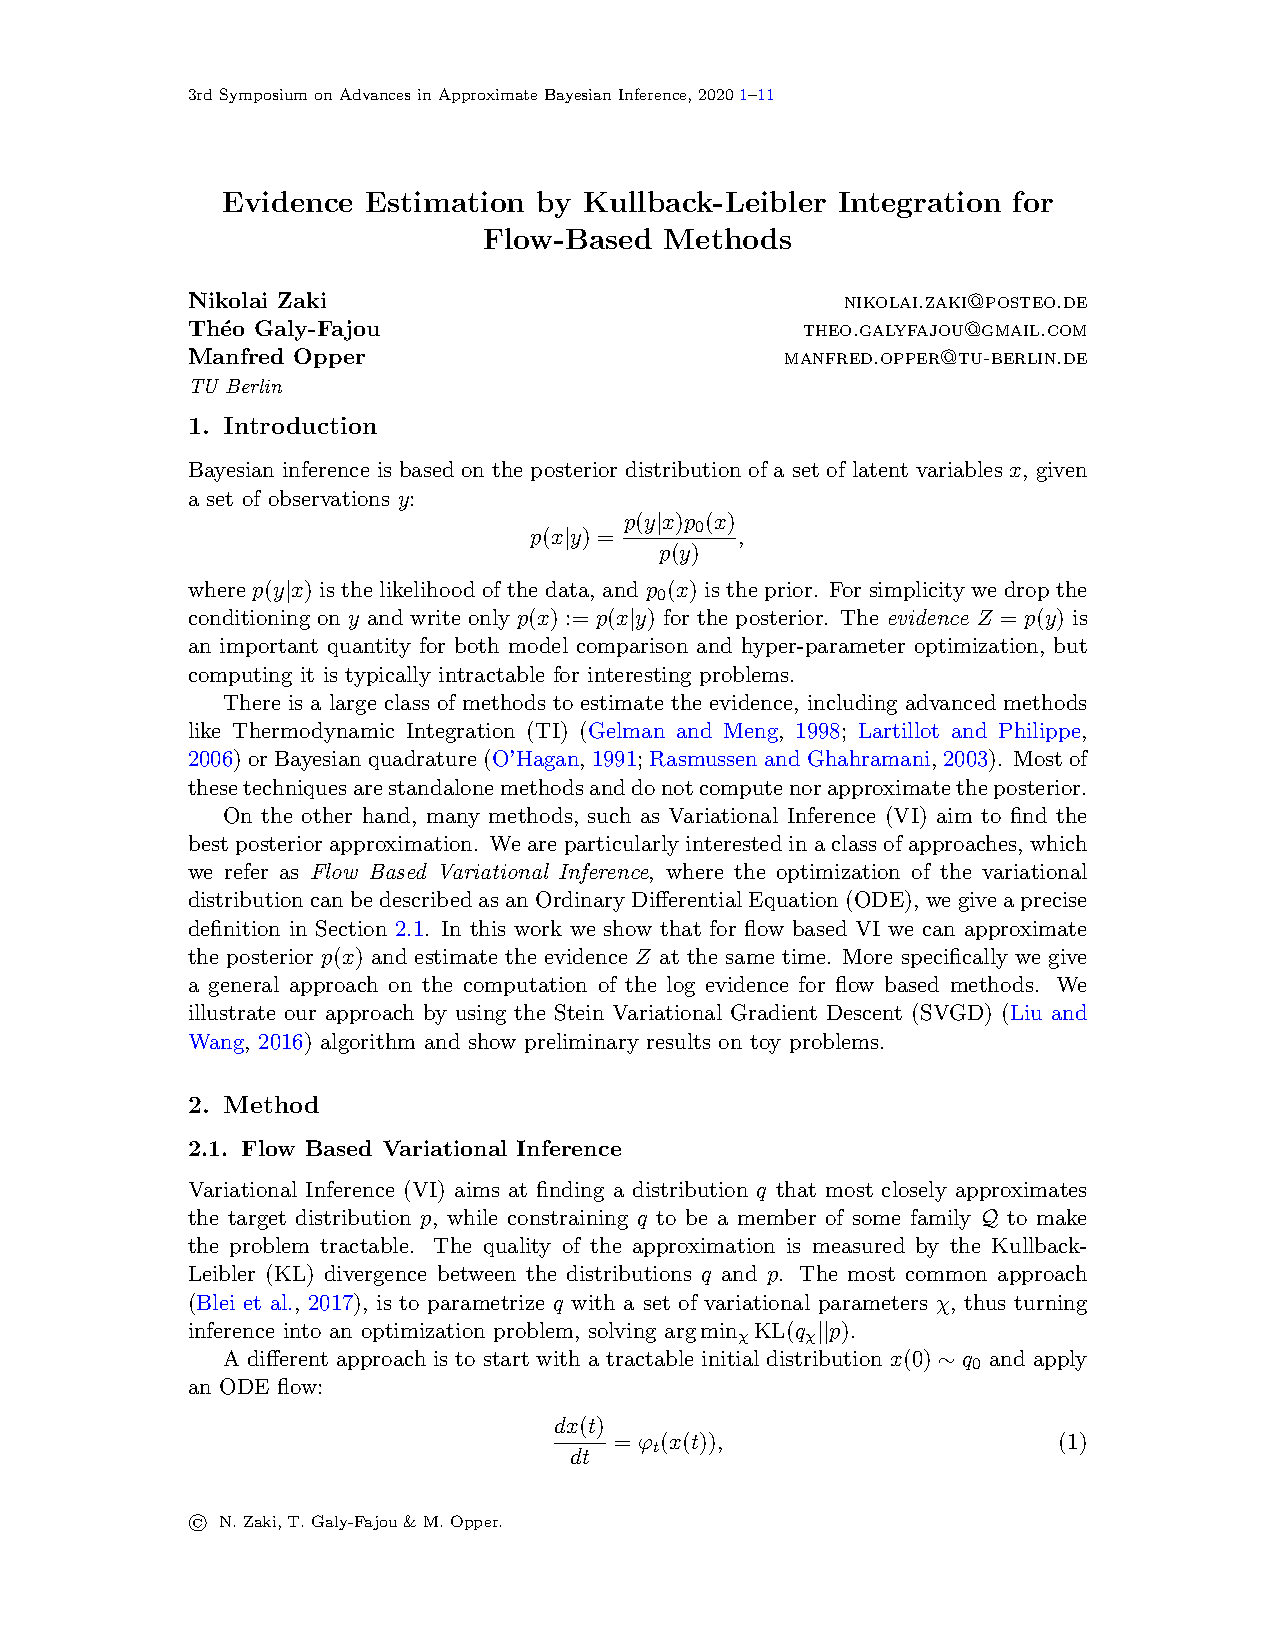
\includepdf[pages=-,pagecommand={},scale=0.95]{./papers/evidence_estimation_by_kullbac.pdf}